%
% Apunte de Sistemas Operativos
% Copyright (C) 2014 Esteban De La Fuente Rubio (esteban[at]delaf.cl)
%
% Permission is granted to copy, distribute and/or modify this document
% under the terms of the GNU Free Documentation License, Version 1.3
% or any later version published by the Free Software Foundation;
% with no Invariant Sections, no Front-Cover Texts, and no Back-Cover Texts.
% A copy of the license is included in the section entitled "GNU
% Free Documentation License".
%
% Link: http://www.gnu.org/copyleft/fdl.html
%

% CAPÍTULO INTRODUCCIÓN
\chapter{Introducción}
El Sistema Operativo (\textit{Operating System, OS}) corresponde a un programa
en ejecución que se encarga de actuar como intermediario entre el usuario y la
máquina. Sus dos principales objetivos corresponden a la \textbf{administración
del hardware} y \textbf{ser una interfaz para el usuario}, de tal forma que este
pueda interactuar con la máquina.

El sistema operativo deberá proveer de un ambiente para ejecutar los programas
del usuario, siendo este \textbf{el único con privilegios de acceso directo al
hardware} y los procesos deberán mediante el sistema operativo acceder a los
recursos disponibles.

Los principales requisitos que se piden al sistema operativo corresponden a ser
\textbf{cómodo} en cuanto a su interfaz y \textbf{eficiente}, de tal forma que
no utilice todos los recursos de la máquina, dejándolos \textit{libres} para los
procesos de los usuarios.

Al estudiar la historia de los sistemas operativos se podrá apreciar como estos
han ido evolucionando en el tiempo. Se verá que inicialmente no existía un
sistema operativo como tal, sino que el hardware era programado directamente
recibiendo los trabajos (\textit{jobs}) que los usuarios deseaban ejecutar. Más
adelante, al aparecer el concepto de un monitor residente, se verá que este
corresponde a un programa que \textbf{siempre se encuentra cargado en memoria
principal}.

\section{Visión general}

En la figura \ref{fig:vision_global} se puede apreciar una visión global del
sistema operativo, en esta se muestran las principales partes que se verán en el
sistema. A continuación se describirá cada uno de estos componentes y como es la
interacción que estos tienen entre sí.

\begin{itemize}

	\item \textbf{Hardware}: recursos disponibles en la máquina, también
	podrán ser dispositivos virtuales, por estos los procesos competirán y
	desearán su uso.

	\item \textbf{Drivers}: código que permite el uso del hardware (o
	dispositivo virtual) al que están asociados.

	\item \textbf{Núcleo}: componente principal del sistema operativo, es el
	intermediario entre aplicaciones y el hardware, se encarga de las tareas
	de administración de la máquina.

	\item \textbf{Llamadas al sistema}: es la forma en que una aplicación
	hace alguna solicitud a un servicio del sistema operativo, generalmente
	con acceso privilegiado por lo cual son accedidas mediante una API.

	\item \textbf{API}: corresponde a una interfaz que pueden utilizar las
	aplicaciones para interactuar con el sistema operativo, las llamadas al
	sistema y eventualmente el hardware disponible, algunas ventajas de esto
	son la abstracción y el escribir menos código.

	\item \textbf{Utilitarios}: aquellas aplicaciones que vienen incluídas
	con el sistema operativo al momento de realizar la instalación, sin
	embargo esto dependerá mucho del sistema operativo propiamente tal y del
	contexto en que cada uno se instala.

	\item \textbf{Aplicaciones}: corresponden al software que se instala
	posteriormente a la instalación del sistema operativo. Generalmente
	serán las aplicaciones que principalmente le interesa ejecutar al
	usuario.

	\item \textbf{Usuario}: usuario del equipo que esta interesado en
	ejecutar sus aplicaciones.

\end{itemize}

\begin{figure}[htbp]
\centering
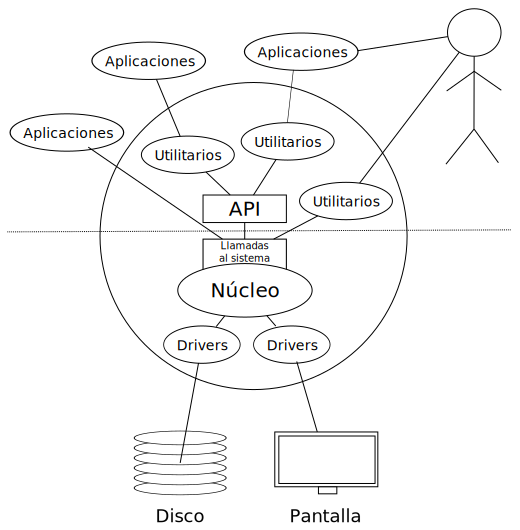
\includegraphics[scale=1.0]{img/C01_introduccion/vision_global.pdf}
\caption{Visión global del Sistema Operativo}
\label{fig:vision_global}
\end{figure}
\FloatBarrier

En la figura \ref{fig:vision_global} se observa una línea divisora entre los
componentes superiores (Aplicaciones, Utilitarios y API) y la parte inferior
(Llamadas al sistema, Núcleo, Drivers y Hardware). Esta división corresponde a
la separación de privilegios necesarios para ser utilizadas. Si bien una
aplicación podría acceder directamente a una llamada a sistema o al hardware
(\textbf{en Unix todo es un archivo}, incluso el hardware) deberá tener los
permisos adecuados para hacerlo. Se hablará más al respecto más adelante en el
capítulo \ref{estructura}.

Una característica importante del sistema operativo, como ya se mencionó antes,
es que es el único proceso que debe estar siempre cargado en memoria principal.
Lo anterior implicará que todo el código del sistema operativo, incluyendo sus
drivers deberán estar cargados siempre en RAM. Imagine que desea tener soporte
para todos los tipos de impresoras disponibles, esto implicaría tener cargado
todos los drivers en la memoria principal por si en algún momento usted la
conecta. Son parte de la estructura del sistema operativo y su diseño la
consideración de diferentes métodos de construcción del núcleo del sistema
operativo, lo que permita cargar por \textit{partes} el mismo, sin tener que
tener cargado todo el código que eventualmente se pueda requerir en la memoria.
Una de estas alternativas es lo que se utiliza en Linux, correspondiente al uso
de módulos donde el núcleo los levanta a medida que los requiere. De esto
también se hablará más en el capítulo \ref{linux_modulos}.

Si bien los recursos con los que se cuenta hoy en día son muy superiores a los
que se contaba cuando comenzaron los sistemas operativos, como se comentará en
el capítulo \ref{historia}, tenga en cuenta que la teoría de sistemas operativos
asociada a los conceptos que se verán en este apunte es muy similar. Existen
avances en tecnologías, pero lo que se abordará en este documento corresponde a
lo tradicional relacionado con sistemas operativos. Por lo cual si usted no
considera problema tener cargado 5, 15, 30 o 200 MB de núcleo RAM, recuerde que
hace unos años los equipos no tenían las mismas capacidades y hace décadas eran
impensables.

\section{Objetivos del sistema operativo}

El sistema operativo debe preocuparse de cumplir diferentes objetivos, estos se
pueden dividir, según el interesado, en \textbf{objetivos del usuario} y
\textbf{objetivos del sistema}.

\subsection{Objetivos del usuario}

Los usuarios finales en general no desean preocuparse por que tipo de hardware
están utilizando. Un usuario que quiere guardar una fotografía en su computador
no le interesa saber en que disco se esta guardando, de que tipo es el disco
(IDE o Sata) o que tipo de sistema de archivos contiene (ext3, reiserfs o xfs),
al usuario le interesa guardar la fotografía.

El objetivo de los desarrolladores estará asociado al fácil desarrollo de
aplicaciones sobre el sistema operativo. Sin tener que, el programador de la
aplicación, llegar a trabajar con lenguaje de bajo nivel o instrucciones
privilegiadas para acceder al hardware de la máquina.

Servicios que serán de interés para los usuarios:
\begin{itemize}

	\item \textbf{Creación de programas}: herramientas para realizar las
	tareas de desarrollo de aplicaciones para el sistema operativo.

	\item \textbf{Ejecución de programas}: administración de los procesos
	que se ejecutan en el sistema.

	\item \textbf{Acceso a los dispositivos de E/S}: simplificación de las
	tareas de uso del hardware, tales como escribir en una pantalla o leer
	datos desde el teclado.

	\item \textbf{Almacenamiento}: administración de los discos, la búsqueda
	de información en estos, su formato y gestión en general.

	\item \textbf{Memoria}: administración del uso de memoria principal
	disponible, así como la asignación de memoria virtual de ser necesario.

	\item \textbf{Detección y respuesta contra errores}: que sea capaz de
	detectar y proteger al sistema frente a eventuales anomalías.

	\item \textbf{Estadísticas}: llevar una recopilación con información
	sobre el uso de los recursos y parámetros generales sobre el sistema.

\end{itemize}

\subsection{Objetivos del sistema}

Desde el punto de vista del sistema la principal preocupación es realizar una
administración eficiente y justa de los recursos de la máquina. Esto significa
que todos sean atendidos en algún momento de tal forma que se les permita
realizar sus operaciones de forma satisfactoria.

El sistema operativo será el encargado de determinar cuando y quién utilizará
cierto recurso del sistema, tal como el procesador, la memoria principal, disco
duro, etc. Y será el encargado de interrumpir al proceso que haga uso del
recurso de tal manera de entregárselo a otro que también lo quiera utilizar.

\section{Servicios ofrecidos}
Históricamente se estudian principalmente tres áreas de la gestión realizada por
el sistema operativo, aquellas relacionadas con los procesos, memoria principal
y secundaria. Adicionalmente se verán en este documento otros aspectos como
protección y seguridad.

\subsection{Gestión de procesos}
Un \textbf{proceso corresponde a un programa en ejecución}, el cual posee
diferentes estados a lo largo de su vida como proceso. Principalmente interesan
los estados listos y ejecución, que corresponden a la espera antes de ser
planificado para entrar a la CPU y el de ejecución de código dentro de la CPU.
Existen otros estados que serán vistos en detalle en el capítulo
\ref{procesos}.

Todo proceso requerirá hacer uso de, al menos, memoria principal y CPU para su
ejecución, por lo cual el sistema operativo deberá ser capaz de asignar estos
recursos de una forma eficiente y justa, de tal forma que todos los procesos
sean servidos según los vayan requiriendo.

Se estudiarán problemas que ocurren por la ejecución de múltiples procesos al
mismo tiempo, concepto conocido como concurrencia, la forma de solucionarlo
mediante sincronización, y algoritmos de planificación que permitirán elegir que
proceso deberá entrar a al cpu.

\subsection{Gestión de memoria principal}
Todo proceso requerirá del uso de memoria principal para su ejecución, en este
espacio de memoria se encontrará no solo el código del programa, sino también
sus datos y su contexto. El sistema operativo deberá asignar, de algún modo,
espacios de memoria para que el proceso los utilice, y si eventualmente el
proceso requiere más espacio poder cumplir con su requerimiento.

¿Qué sucede si no disponemos de más memoria principal? La primera idea, sería
decir que no podemos iniciar más procesos, lo cual sería cierto, sin embargo se
discutirá el método de memoria virtual el cual permite utilizar un dispositivo
de memoria secundaria para ``obtener memoria'' para los procesos.

\subsection{Gestión de memoria secundaria}
El sistema operativo debe ser capaz de almacenar datos en medios de memoria
secundaria, la cual es permanente, a diferencia de la memoria principal que es
volátil. Se deberá preocupar de la mantención de una estructura de archivos y de
poder realizar operaciones sobre esta estructura de tal forma que las
aplicaciones no se preocupen de escribir \textit{físicamente} el archivo que
desean guardar en el disco.

\section{Ejercicios y preguntas}
\begin{enumerate}

	\item Explique los objetivos del sistema operativo.

	\item Explique los componentes de la visión general del sistema
	operativo y como se relacionan entre si. Realice diagrama.

	\item ¿Por qué los objetivos del usuario y del sistema operativo no
	siempre son compatibles?.

	\item ¿Cuáles son los servicios básicos que el sistema operativo debe
	proveer?.

	\item ¿Cuándo se encuentra cargado el sistema operativo en RAM?.

\end{enumerate}

\section{Referencias}
\begin{itemize}

	\item Sistemas Operativos, Segunda Edición, Andrew Tanenbaum, Capítulo 1.1.

\end{itemize}
